\chapter{Introduction}
A first definition of \ml by T. Mitchell is the following one:
\begin{center}
	\textit{A computer program is said to learn from experience E with respect to some class of tasks T and performance measure P, if its performance at tasks in T, as measured by P, improves with experience E.}
\end{center}
That is, \ml builds a model that allows the computer to learn from experience, but does not solve the problem directly (as it's not always possible). \newline
For a well-posed learning problem there a few key components:
\begin{itemize}
	\item \textbf{Task}: For example recognising characters;
	\item \textbf{Performance measure}: to evaluate the learned system, that is the way the success of the predictors is measured (for example the number of misclassified characters).
	\item \textbf{Training experience}: to train the learning system, that is what is given to the system as experience E so that the algorithm can improve. The easiest way to do so is to give a training set made of couples.
\end{itemize}
\section{Designing a machine learning system}
The following steps should be followed when designing a \ml system:
\begin{itemize}
	\item Formalize the learning task;
	\item Collect data;
	\item Extract features;
	\item Choose class of learning models;
	\item Train model;
	\item Evaluate model.
\end{itemize}
\subsection{Formalize the learning task}
As a first step, it's important to define the task that the learning system should address, for example recognizing handwritten characters.\newline
Often the main task can be divided in smaller tasks such that the problem gets easier to be solved. Considering the example before, it could be split in:
\begin{itemize}
	\item Segment the image into words and then each word into characters.
	\item Identify the language of the writing.
	\item Classify each character into the language alphabet.
\end{itemize}
At last to define the task, one should also choose an appropriate performance number for evaluating such system, for example the number of misclassified characters could be a good performance measure. 
\subsection{Collect data}
Since the \ml system needs to learn from something, we need a so called training set, that is a set of example written in a \textit{machine readable format}.\newline
For such reason, often the data require some manual intervention, for example in labelling, in order to have a so called supervised learning, that is the training set is formed of a couple containing the initial data and also the correct result that the system should get. This, though, could be quite expansive to be achieved so a much cheaper learning mode is being used, the so called semi-supervised learning, where supervised data is mixed to data which does not have the expected result nor it's labeled. 
\subsection{Extract features}
Not all the data that is given is really useful and instead sometime is harmful. For this reason a relevant set of feature should be extracted from all the data, that is fundamental information for the input in order for the algorithm to give the correct solution. To do this the best way possible, some prior knowledge is usually necessary. \newline
Mind that:
\begin{itemize}
	\item Too few features could miss some relevant information preventing the system from learning in a correct way.
	\item Too many feature could heavy the system too much and the training phase could take a lot of time.
	\item Including noisy features complicates the training phase as the algorithm needs to learn to avoid these. 
\end{itemize}
\subsection{Model class}
Many model classes are available and choosing the best one is important. For example a binary classification, that is a simple linear model that separates data in to two classes. 
\begin{center}
	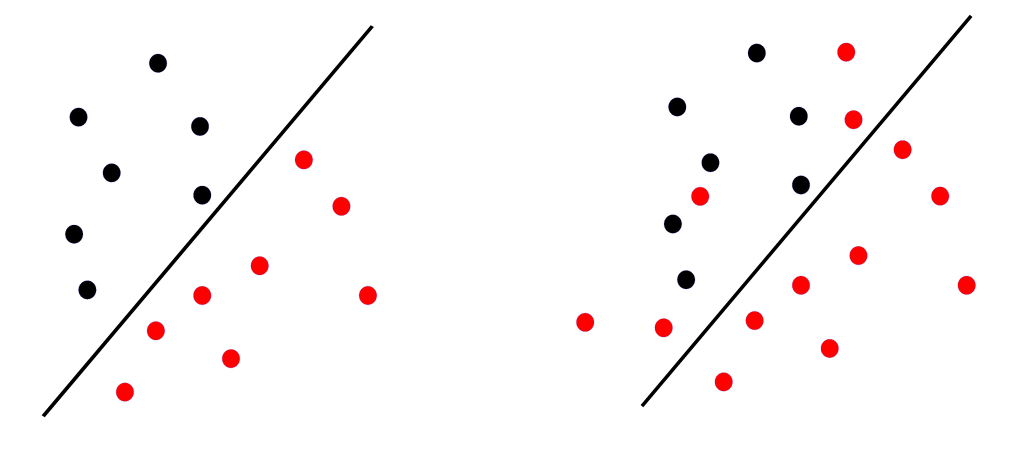
\includegraphics[width=\linewidth]{BinaryClassifier}
\end{center}
We call features all the points, that is the example given, and classes the colors, that is the supposed result of the algorithm. It's easy to notice that a binary classifier works as a separator that is a feature can have a class or another. Not always is possible to define a linear function that separates the features, so in some cases a more complex model can be used. 
\begin{center}
	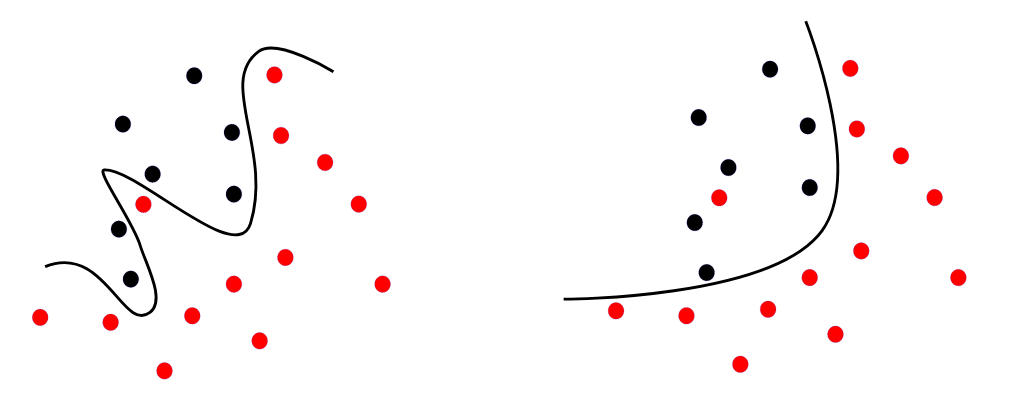
\includegraphics[width=\linewidth]{BinaryClassifier2}
\end{center}
It's possible to notice that in this case the red feature in the middle of all the black ones introduce a lot fo noise. Mind that we still are in a training phase and we do not mind for some false positive o negatives, we want our system to be good in real life not in the training set. If now a complex model is designed, such as the one on the left, the system doesn't learn how to recognize noise and to get rid of it. This problem is called overfitting and should be avoided. \newline
Quindi non vogliamo che il nostro sistema semplicemente memorizzi i dati del training, ma che riesca a generalizzarli. 
\subsection{Learning settings}
We have already talked about possible types of learning, such as supervised or semi-supervised learning, but they are not all that there is.  
\begin{itemize}
	\item \textbf{Supervised learning}: the learner is given a series of pair where one element is input and one is the correct output. What the algorithm should do is to learn a function $f$ that maps each input to output. Formally given a set of inputs $\mathcal{X}$ and outputs $\mathcal{Y}$, the learner is provided with couples $(x_i, y_i)\in \mathcal{X}\times\mathcal{Y}$ in order to create a \textit{model} $f:\mathcal{X}\mapsto \mathcal{Y}$. Since each example need to have a correct output, usually a domain expert is involved in \textit{labelling} the couples. 
	\item \textbf{Unsupervised learning}: the learner is provided with a set of input examples $\mathcal{X}$ but without any labelling information, that is no output. In this case the learner models training examples, for instance grouping examples into clusters according to their similarity. 
	\item \textbf{Semi-supervised learning}: this stays in the middle of the formers. As in supervised learning, the learner is provided with a set of input/output pairs: $(x_i, y_i)\in \mathcal{X}\times\mathcal{Y}$. The difference is that the set of inputs is usually much larger than the outputs one providing additional unlabelled examples. As in supervised learning the goal is to find a model $f$ that maps input into outputs: $f:\mathcal{X}\mapsto\mathcal{Y}$. The unlabelled data is exploited in order to improve performance, for example by forcing the model to produce similar outputs for similar inputs. 
	\item \textbf{Reinforcement learning}: in this type of learning, the actor is not provided anymore with inputs and outputs, but is given a set of possible states $\mathcal{S}$ and a set of possible actions $\mathcal{A}$ that allows it to move to the next state. When the learner performs an action $a$ from a state $s$, it is given a reward $r(s,a)$. The task is to learn a policy allowing to choose for each state s the action a maximizing the overall reward. One problem is that the reward may not always be immediate but instead might be delayed. If this is the case, the learner needs to find the right trade-off between exploitation and exploration. An example of delayed reward is chess where the learner knows its reward only at the end.
\end{itemize}

\subsubsection{Choice of learning algorithm}
The choice of the algorithm to use is based on the knowledge we have of the data:
\begin{itemize}
	\item Full knowledge of probability distribution of data: Bayesian decision theory.
	\item Form of probabilities known, parameters unknown: parameter estimation from training data.
	\item Form of probabilities unknown, training examples available: do not model input data (generative methods), learn a function predicting the desired output given the input.
	\item Form of probabilities unknown, training examples unavailable (only inputs): unsupervised methods, cluster examples by similarity.
\end{itemize}
\subsubsection{Learning tasks}
For what concerns the supervised learning, possible tasks are: 
\begin{itemize}
	\item \textit{Binary}: it's the easiest task, or the element belongs to a class, or to the other.
	\item \textit{Multiclass}: an element can belong to one of the set of the class.
	\item \textit{Multilabel}: given $n$ possible classes, the example can be assigned to a subset of $m\leq n$ classes.
	\item \textit{Regression}: in this case a real value is predicted, for example the biodegradation rate of a molecular compound.
	\item \textit{Ordinal regression} (ranking): a set of examples is ordered according to their relative importance with respect to the task, for example ordering email according to their urgency.
\end{itemize}
For what concerns unsupervised learning:
\begin{itemize}
	\item \textit{Clustering}: data is divided into groups in order to have homogeneous elements in each group and so that each group is enough different from the others.
	\item \textit{Dimensionality reduction}: in this case there are many features and the aim is to reduce their dimensionality maintaining as mach information as possible.
	\item \textit{Novelty detection}: given a certain distribution of data, the aim of this task is to find all the element that are novel, that is don't respect the distribution. This approach is used for example in network traffic analysis in order to detect anomalous traffic that indicates a possible attack.
\end{itemize}
%
%
\subsection{Train Model}
Training a model implies searching through the space of possible models (aka hypotheses) given the chosen model class.\newline
Such search typically aims at fitting the available training examples well according to the chosen performance measure. \newline
However, the learned model should performe well on unseen data, \textbf{generalization}, and not simply memorize training examples, \textbf{overfitting}.\newline
Different techniques can be used to improve generalization, usually by trading off model complexity with training set fitting.
%
%
\subsection{Evaluate Model}
Once a fitting model is found, it needs to be evaluated on its ability to generalize to unseen examples. \newline
For this reason there is the need to have a set of data that is different from the training one. Usually from a unique dataset, two are derived, one for training and one for evaluation.


